\documentclass{standalone}
\usepackage{tikz}
\usepackage{amsmath}

\begin{document}

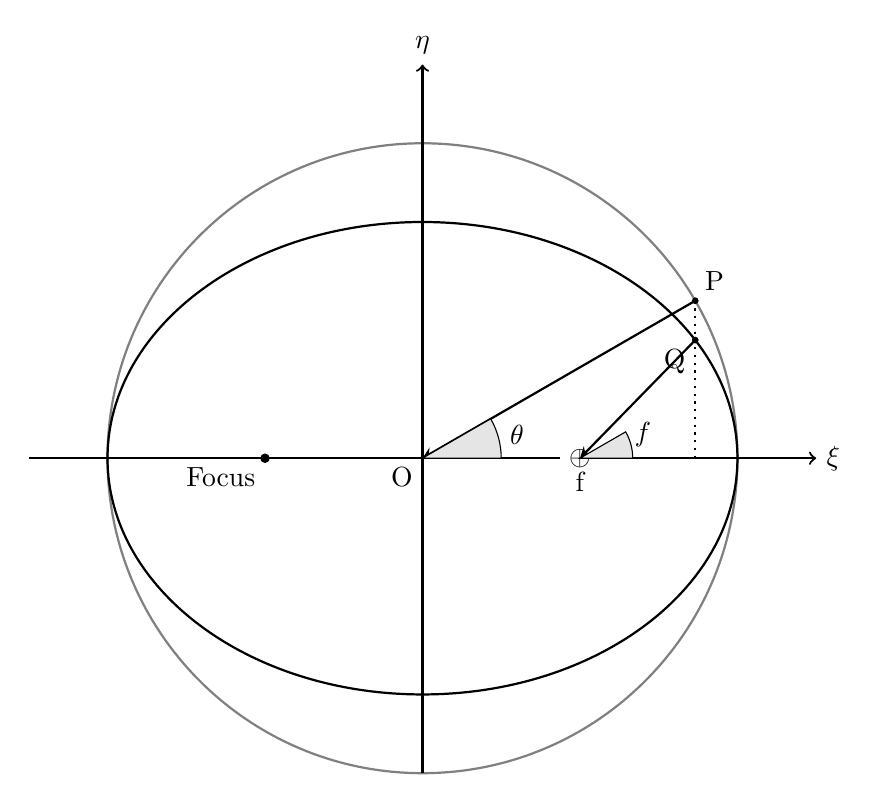
\begin{tikzpicture}

    % Define parameters
    \def\radius{4} % Radius of the circle
    \def\angle{30} % Angle theta (pi/6) in degrees
    \def\focusX{2} % Focus of the ellipse (positive x-axis)
    \def\semiMajor{4} % Semi-major axis of the ellipse
    \def\semiMinor{3} % Semi-minor axis of the ellipse

    % Circle (gray)
    \draw[thick, gray] (0,0) circle(\radius cm);

    % Ellipse (black)
    \draw[thick, black] (0,0) ellipse (\semiMajor cm and \semiMinor cm);

    % Axes
    \draw[->, thick] (-5,0) -- (5,0) node[anchor=west] {$\xi$}; % Horizontal axis
    \draw[->, thick] (0,-4) -- (0,5) node[anchor=south] {$\eta$}; % Vertical axis

    % Origin (O)
    \node at (0,0) [below left] {O};

    % Earth symbol at positive focus (f) with white background
    \node[fill=white] at (\focusX, 0) {$\oplus$};
    \node at (\focusX, -0.3) {f};

    % Mark the other focus (negative focus)
    \filldraw (-\focusX,0) circle(1.5pt) node[below left] {Focus};

    % Point P on the circle (corresponding to theta = pi/6)
    \coordinate (P) at ({\radius*cos(\angle)}, {\radius*sin(\angle)});
    \filldraw (P) circle(1pt) node[anchor=south west] {P};

    % Point Q on the ellipse (Q = (a cos theta, b sin theta))
    \coordinate (Q) at ({\semiMajor*cos(\angle)}, {\semiMinor*sin(\angle)});
    \filldraw (Q) circle(1pt) node[anchor=north east] {Q};

    % Arrow from O to P (Op) with tail at the origin and head at P
    \draw[->, thick, stealth-] (0,0) -- (P) node[midway, above right] {};

    % Arrow from f to Q (fq) with tail at the focus and head at Q
    \draw[->, thick, stealth-] (\focusX, 0) -- (Q) node[midway, below right] {};

    % Dotted line from P to Q
    \draw[dotted, thick] (P) -- (Q);

    % Dotted line from P to the horizontal axis
    \draw[dotted, thick] (P) -- ({\radius*cos(\angle)}, 0);

    % Shaded angle for POp (angle = theta)
    \filldraw[fill=gray!20] (0,0) -- (1,0) arc[start angle=0, end angle=\angle, radius=1cm] -- cycle;
    \node at (1.2, 0.3) {$\theta$};

    % Shaded angle for Pfq (angle subtended by Pfq)
    \filldraw[fill=gray!20] (\focusX, 0) -- ++(0.67,0) arc[start angle=0, end angle=\angle, radius=0.67cm] -- cycle;
    \node at (2.8, 0.3) {$f$};

\end{tikzpicture}

\end{document}
